 \author{Nguyễn Quốc Dương, GVHD: TS. Lê Thanh Bính.}
 \documentclass[12pt, a4paper,oneside]{book}
 \usepackage{amsmath, amssymb, latexsym, amscd, amsthm,amstext}
 \usepackage{graphics}
 \usepackage{color, colortbl}            % Màu trong bảng
 \usepackage{varwidth}               
 \usepackage{multicol}
 
 \usepackage{hyperref}    
 \usepackage[utf8]{vietnam}
 \usepackage{anysize}							
 \marginsize{3cm}{2cm}{2cm}{2cm}				%\marginsize{left}{right}{top}{bottom}
 %\papersize{width}{height}	
 \usepackage{listings}
 \usepackage{booktabs}
 \usepackage{siunitx}
 \usepackage{longtable}                  % Tạo bảng dài
 \usepackage{tocbibind}
 \usepackage[toc,page]{appendix}         % Tô màu khung - nền - chữ
 \usepackage{graphicx}
 \usepackage{longfbox}		          	% Tạo hộp văn bản - box	
 \title{Sections and Chapters}
 \usepackage{multicol}
 \usepackage{wrapfig}  
 \usepackage{enumerate}
 \usepackage{dsfont}
 \usepackage{commath}
 \renewcommand{\baselinestretch}{1.3} 
 \renewcommand{\figurename}{\bf Hình}
 %%========================================
 \newtheorem{theo}{\bf Định lý}[section]
 \newtheorem{coro}[theo]{\bf Corollary}
 \newtheorem{lemm}[theo]{\bf Bổ đề}
 \newtheorem{prop}[theo]{\bf Mệnh đề}
 \newtheorem{algo}[theo]{\bf Thuật toán}
 \newtheorem{conj}[theo]{\bf Conjecture}
 
 \theoremstyle{definition}
 \newtheorem{dn}[theo]{Định nghĩa}
 \newtheorem{dl}[theo]{Định lý}
 \newtheorem{tc}[theo]{Tính chất}
 \newtheorem{vd}[theo]{\it Ví dụ}
 \newtheorem{cy}[theo]{\it Chú ý}
 \newtheorem{nx}[theo]{\it Nhận xét}
 \newtheorem{pt}{\it Phân tích}
 %\def\R{\mathbb{ R}}                        %Các kí hiệu tập hợp
 %\def\re{\mbox{\rm \texttt{Re}}}            %Định nghĩa từ viết tắt
 %\def\im{\mbox{\rm \texttt{Im}}}
 %=========================================
 
 \newcommand{\seq}[1]{\left<#1\right>}
 \makeatletter
 \def\ps@myheadings{%
 	\def\@evenhead{\hfil\thepage\hfil}
 	\def\@oddhead{\hfil\thepage\hfil}}
 \makeatother 
 \marginsize{3cm}{2.5cm}{2cm}{2cm}
 \marginsize{3cm}{2.5cm}{2cm}{2cm}
 \DeclareMathOperator{\sgn}{sgn}
 \DeclareMathOperator{\rank}{rank}
 \pagestyle{myheadings}
 \newcommand{\blue}[1]{\textcolor{blue}{#1}}
 \newcommand{\red}[1]{\textcolor{red}{#1}}
 %=======================
 
 \DeclareUnicodeCharacter{2212}{-}
 \setlength{\parindent}{1 cm}
 \usepackage{cases}
 %=======================
 
 \definecolor{dkgreen}{rgb}{0,0.6,0}             % Môi trường chứa code
 \definecolor{gray}{rgb}{0.5,0.5,0.5}
 \definecolor{mauve}{rgb}{0.58,0,0.82}
 \lstset{frame=tb,
 	language=R,
 	aboveskip=3mm,
 	belowskip=3mm,
 	showstringspaces=false,
 	columns=flexible,
 	basicstyle={\small\ttfamily},
 	numbers=none,
 	numberstyle=\tiny\color{gray},
 	keywordstyle=\color{blue},
 	commentstyle=\color{dkgreen},
 	stringstyle=\color{mauve},
 	breaklines=true,
 	breakatwhitespace=true,
 	tabsize=3}
 %=============================
\begin{document}
\begin{center}
\textbf{ỨNG DỤNG SHINY KẾT HỢP VỚI MÔ HÌNH ARIMA ĐỂ PHÂN TÍCH ĐẠI DỊCH COVID-19}
\end{center}
\begin{center}
\textbf{Nguyen Quoc Duong$^{1, *}$}, \textbf{Le Thanh Binh$^{2}$}
\end{center}
\begin{center}
\textit{$^{1}$Khoa Sư Phạm, Trường Đại học Quy Nhơn, Việt Nam}\\
\textit{$^{2}$Khoa Toán và Thống kê, Trường Đại học Quy Nhơn, Việt Nam}
\end{center}
\begin{center}
\textit{$^{*}$Tác giả liên hệ: Email: nguyenquocduongqnu1999@gmail.com}
\end{center}
\textbf{TÓM TẮT}

Trực quan hóa dữ liệu là một công cụ quan trọng để khám phá và truyền đạt những phát hiện trong nghiên cứu y học và đặc biệt là trong giám sát dịch tễ học. Trong bài nghiên cứu này, chúng tôi sử dụng gói lệnh shiny và mô hình ARIMA để xây dựng một website dự báo khuynh hướng dịch bệnh COVID-19. Dữ liệu phân tích về dịch COVID-19 tại mỗi quốc gia trên toàn thế giới được cập nhật hằng ngày từ hệ thống của ứng dụng COVID19 Dashboard.\\
\textbf{Keywords:} ARIMA, Shiny app, COVID-19, auto.arima, forecast.
\newpage
\begin{center}
	\textbf{SHINY APPLICATION WITH ARIMA MODEL EVALUATE PANDEMIC COVID-19}
\end{center}
\begin{center}
	\textbf{Nguyen Quoc Duong$^{1, *}$, Le Thanh Binh$^{2}$}
\end{center}
\begin{center}
	\textit{{$^{1}$Faculty of Education, Quy Nhon University,\\ 170 An Duong Vuong, Quy Nhon, Binh Dinh, Viet Nam}}\\
	\textit{$^{2}$Faculty of Mathematics and Statistics, Quy Nhon University,\\ 170 An Duong Vuong, Quy Nhon, Binh Dinh, Viet Nam}
	
\end{center}
\textbf{ABSTRACT}

Data visualization is an important tool for exploring and communicating findings in medical research, and specially in epidemiological surveillance. For forecast of time series, ARIMA model is one of the best modeling techniques. In this study, we aim to use the shiny package and the ARIMA model in order to creating a website for predicting trend of the COVID-19 disease  in all over the world. The COVID-19 Dashboard app systematically produces daily updated data analysis of COVID-19 pandemic.\\
\textbf{Keywords:} ARIMA, Shiny app, COVID-19, auto.arima, forecast.
\vskip 0.5cm
\noindent 
{\bf 1. INTRODUCTION}

Coronavirus disease 2019 (COVID-2019) has been recognized as a global threat, and several studies are being conducted using various mathematical models as SEIR (susceptible - exposed - infectious - recovered), FLM (functional linear model), ETS (Exponential Smoothing State Space),  \dots  combined with shiny app to predict the probable evolution of this epidemic \cite{1}. Besides, several studies have used ARIMA model to fit and predict changing trends in COVID-19 disease. Alzahrani SI and et al. applied ARIMA model to forecasting the spread of the COVID-19 pandemic in Saudi Arabia \cite{2}. In addition, Lutfi Bayyurt and Burcu Bayyurt used ARIMA model to forecast COVID-19 Cases and Deaths \cite{3}. Furthermore, Nguyen Quoc Duong and et al. applied ARIMA model to predicting the Pandemic COVID-19 \cite{4}. Therefore, ARIMA model seem to be a good tool that can help the health authorities to monitor and assess the spread of the outbreak.

R is one of the tools that has relevant importance for epidemiologists, and had quick search function can enable users to get many R libraries devoted to outbreak management and analysis. Consequently, by combining the ARIMA model and shiny package to create a website to track disease trends for each country. This study aims to develop a prediction model app for the daily total confirmed new cases, total deaths new cases and total recovered new cases based on ARIMA model.
\vskip 0.5cm
\noindent 
{\bf 2. METHODOLOGY}\\
{\bf 2.1. SOFTWARE AVAILABILITY AND REQUIREMENTS}\\

The COVID-19 Dashboard app has been developed in RStudio, version 1.2.5033, using the Shiny package, version 1.4.0. Shiny offers the ability to develop a graphical user interface (GUI) that can be run locally or deployed online. Last is particularly beneficial to show and communicate updated findings to a broad audience. All the analyses have been carried out using R, version 4.0.1.

The app has a friendly structure based on menus to shown data visualization for each of the analyses implemetned: overview and predicting trend using ARIMA Model (Figure \ref{D1} and Figure \ref{D2}).
\begin{figure}[!htb]
	\centering
	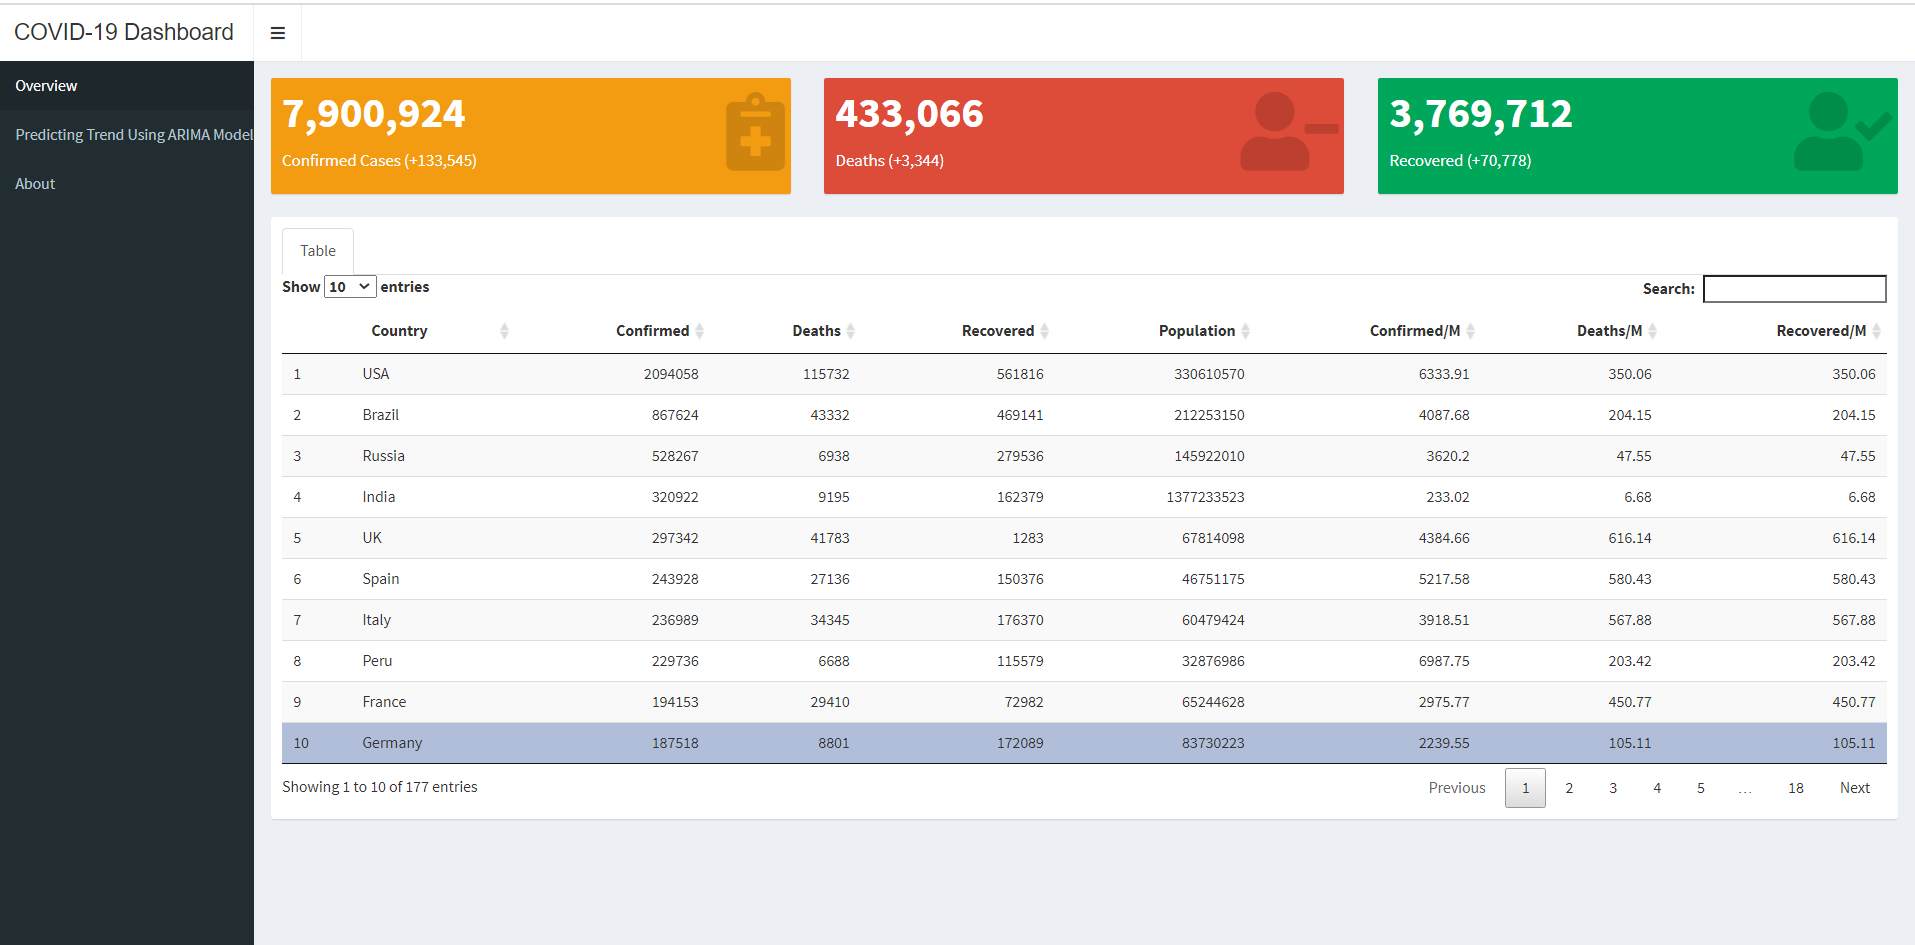
\includegraphics[width=1\linewidth,height=7.7cm]{anh/D1}
	\vskip-4mm 
	\caption{Tag overview (15/06/2020)}  
	\label{D1}
\end{figure}
\begin{figure}[!htb]
	\centering
	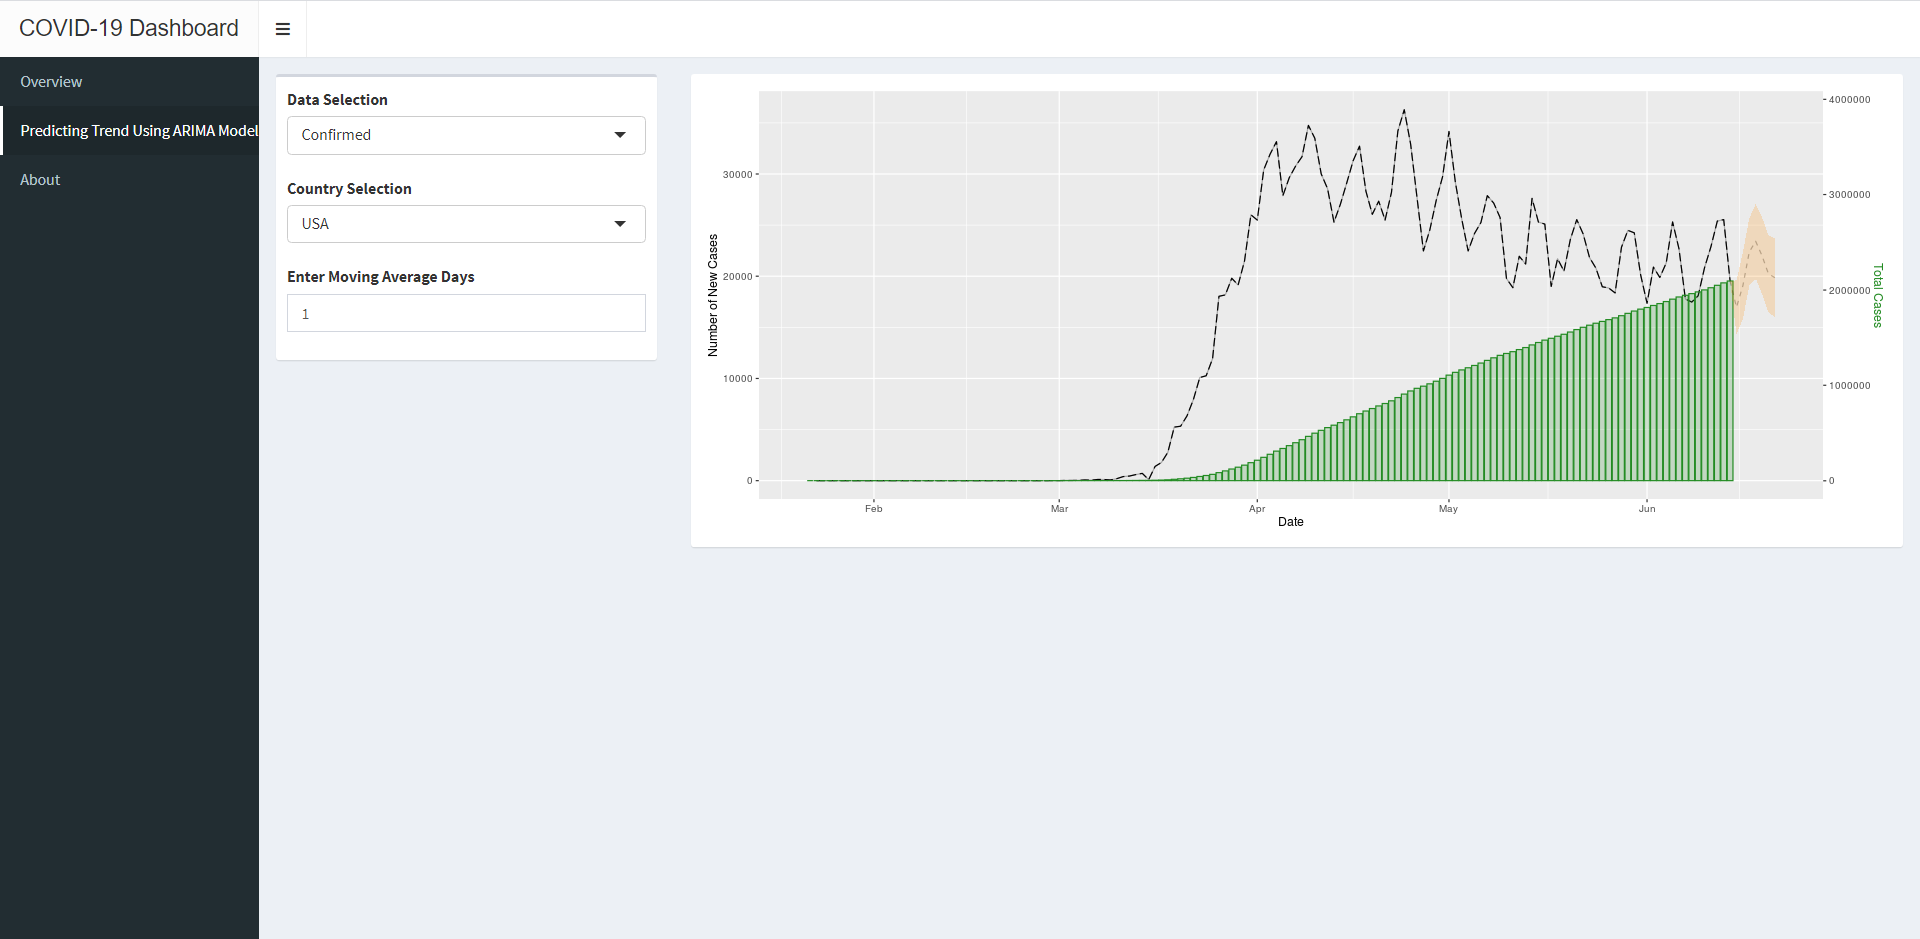
\includegraphics[width=1\linewidth,height=7.7cm]{anh/D2}
	\vskip-4mm 
	\caption{Tag predicting trend using ARIMA model (15/06/2020)}.  
	\label{D2}
\end{figure}

The app has an automated process to update data and all analyses every time a user connects to the app. It is available online at the following link: \url{https://nguyenquocduong.shinyapps.io/NCKH/}.
\vskip 0.5cm
\noindent 
{\bf 2.2. DATA SOURCES}

To ensure the accuracy and the reliability of the tracker's content, the website's server retrieves the newest data from the COVID-19 data repository by the Center for Systems Science and Engineering at Johns Hopkins University when any user tries to load the web page. The data repository is regulated by the Johns Hopkins University Center for Systems Science and Engineering and supported by the ESRI Living Atlas Team and the Johns Hopkins University Applied Physics Lab.

According to the documentation of the repository, the data source is being updated in real-time numerous times throughout the day, and the validity of the data is verified by researchers at Johns Hopkins University. The content displayed in the overview feature is therefore derived from a real-time and reliable data source.
\vskip 0.5cm
\noindent 
{\bf 2.3. ARIMA MODEL}

ARIMA was first formed by Box and Jenkins, (1970) \cite{6, 7}. The general equation of successive differences at the $d$  difference of $X_t$ is briefly expressed as equation (\ref{eq1}), (\ref{eq2}) and (\ref{eq3}).
\begin{equation}
	\Delta^{d}X_t = (1-B)^{d}X_t,
	\label{eq1}
\end{equation}
where $d$ is the difference degree and B is the backshift operator. The successive difference at onetime lag equals according to equation (\ref{eq2}).
\begin{equation}
\Delta^{1}X_t = (1-B)X_t = X_t - X_{t-1}.
\label{eq2}
\end{equation}

In this situation, the general non-seasonal ARIMA($p$, $d$, $q$) is as equation (\ref{eq3}).
\begin{equation}
\phi_p(B)W_t = \theta_q(B)e_t,
\label{eq3}
\end{equation}
where $\phi_p(B)$ is an auto-regressive operator of order $p$, $\theta_q$  is a moving average operator of order $q$, and $W_t = \Delta dX_t$.

To select the appropriate parameter that can be applied to the ARIMA model, model selection criteria was applied as \textit{Akaike's Information Criterion} (AIC) (Akaike, 1974). According to Akaike, (1974) and Mohammed et al. (2015), a good model exhibits the lowest AIC value \cite{6}. As described by Akaike (1974), AIC is expressed as equation (\ref{eq4}).
\begin{equation}
AIC = -2\ln(L)+ 2k,
\label{eq4}
\end{equation}
where $L$ is the value of the likelihood and $k$ is the number of estimated parameters in the model. 

R also has a package called forecast, which contains many forecasting functions for time series and linear models \cite{7, 8}. It also contains a very useful function called auto.arima, which return the best ARIMA model according to either AIC value. The auto.arima() function uses a variation of the Hyndman-Khandakar algorithm (Hyndman \& Khandakar, 2008) \cite{8}. The function conducts a search over possible models within the order constraints provided.

For every given time series, as a part of the output from the auto.arima() function, the 95\% intervals are taken to plot the transparent orange ribbon around the mean prediction. The 95\% confidence intervals for ARIMA forecasts are computed as
\begin{align*}
	\hat{y}_{T+h|T} \pm 1.96\sqrt{v_{T+h|T}},
\end{align*}
where $v_{T+h|T}$ refers to the variance of $y_{T+h|y_1, \dots, y_T}$.
\vskip 0.5cm
\noindent 
{\bf 3. APPLICATIONS}\\
\noindent 
{\bf 3.1 Overview}

According to the Figure \ref{D1}, the top of the page has three odometer boxes to display the total confirmed cases, total deaths, and total recovered cases along with their respective daily new counts. 

In addition, the display window has the viewing option of data tables. All tables can be interactively sorted by clicking on column names. The data table provides the users with the flexibility to explore and search for data of their interest.

In brief, the purpose of this feature is to provide the audience with an aggregated view of the severity of COVID-19 in different locations and inform the audience of the latest status of the disease at a first glance \cite{9, 10}.\\
\noindent 
{\bf 3.2 Predicting trend using ARIMA model}

Observing Figure \ref{D2}, the display window shows visualizations of a bar plot of the total cases, a line plot of daily new cases with respect to time along with its moving average, and a 7-days interval estimation of daily new cases.

In short, the visualization is presented in a dual-axis plot. The gray line in the back represents the number of new cases while the dotted black line represents the moving average of the number of new cases, and they correspond to the left vertical axis. The green bar plot represents the accumulated total cases, and it corresponds to the right vertical axis.

Consequently, the purpose of this feature is to inform the audience with insights into the trend of the spread of the disease in each individual country. From this feature, we can observe various trends and patterns as countries around the globe have been reacting differently to mitigate the spread of COVID-19. For example,  Italy has implemented a relatively strict country-level lockdown policy, and it is being reflected from their trend plot. According to the Figure \ref{D3}, the number of new cases has been gradually decreasing, the rate of decrease is relatively fast. Similarly, we can choose deaths data or recovered data.
\begin{figure}[!htb]
	\centering
	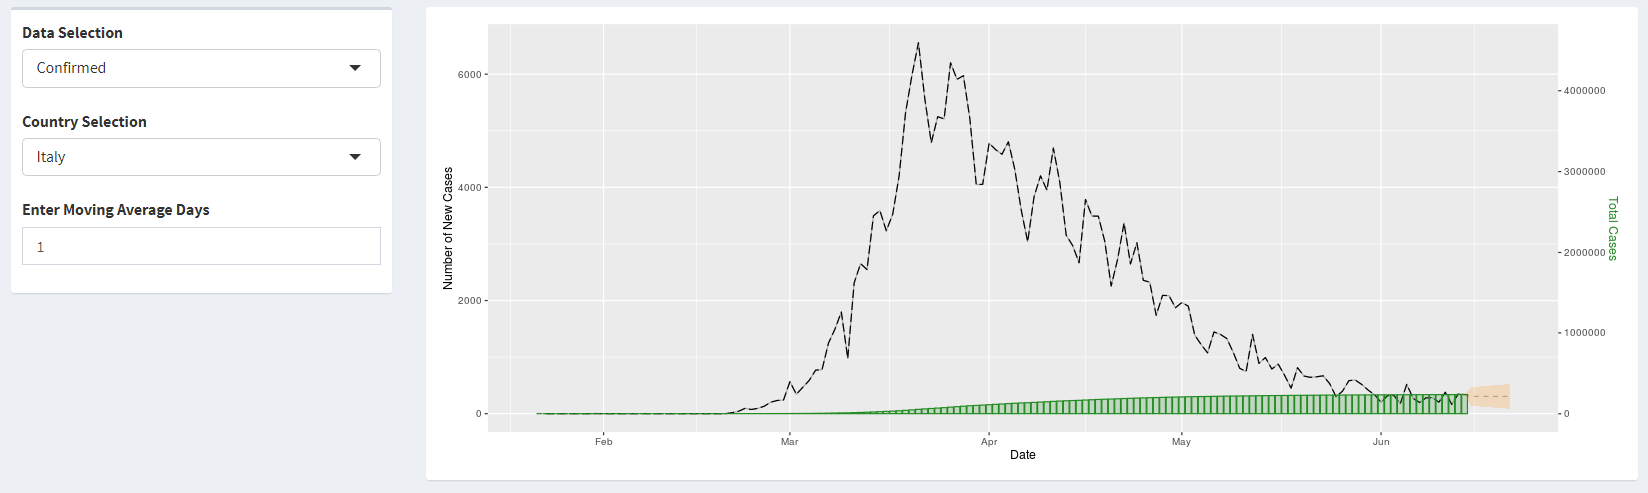
\includegraphics[width=1\linewidth,height=7.7cm]{anh/D3}
	\vskip-4mm 
	\caption{Predicting trend of Italy using ARIMA model (15/06/2020)}.  
	\label{D3}
\end{figure}
\vskip 0.3cm
\noindent 
{\bf 4. CONCLUSIONS}

The COVID-19 Dashboard application presents a set of tools for updated analysis and graphic visualization that can be very useful for a better understanding of the evolution of the COVID-19 epidemic in all the world and its epidemiological surveillance.

In summary, this application, easy to use, come to fill a gap in this particular scenario for the visualization of epidemiological data for the COVID-19  epidemic in all the world.
\clearpage
\begin{thebibliography}{99}
	\bibitem{1} Antoine Soetewey, \textbf{\textit{Top 100 R resources on Novel COVID-19 Coronavirus}}, Towards Data Science, \url{https://bitly.com.vn/CzdP3}.
	\bibitem{2} Alzahrani SI and et al., \textbf{\textit{Forecasting the spread of the COVID-19 pandemic in Saudi Arabia using ARIMA prediction model under current public health interventions}}, Journal of Infection and Public Health, 2020, \url{http://dx.doi.org/10.1101/2020.03.30.20046227}.
	\bibitem{3} Lutfi Bayyurt and Burcu Bayyurt, \textbf{\textit{Forecasting of COVID-19 Cases and Deaths Using ARIMA Models}}, The preprint server for health sciences, 2020, \url{https://doi.org/10.1101/2020.04.17.20069237}.
	\bibitem{4} Nguyen Quoc Duong and et al., \textbf{\textit{Predicting the Pandemic COVID-19 using ARIMA Model}}, VNU Journal of Science: Mathematics-Physics, 2020.
	\bibitem{5} R. H. Shumway and D. S. Stoffer, \textbf{\textit{Time Series Analysis and Its Applications}}, Springer Publisher, 2006.
    \bibitem{6} G. E. P. Box, G. M. Jenkins, G. C. Reinsel and G. M. Liung, \textbf{\textit{Time Series Analysis: Forecasting and Control, $5^{th}$ edition}}, Publisher Wiley, 2016.
    \bibitem{7} R. J. Hyndman and G. Athanasopoulos, \textbf{\textit{Forecasting: Principles and Practice, $2^{nd}$ edition}}, OTexts Publisher, 2018.
    \bibitem{8} Rob J. Hyndman and Yeasmin Khandakar, \textbf{\textit{Automatic Time Series Forecasting: The forecast Package for R}}, Journal of Statistical Software, 2018, Volume 27, Issue 3.
    \bibitem{9} Keon-Woong Moon, \textbf{\textit{Learn ggplot2 Using Shiny App}}, Springer, 2017.
    \bibitem{10} Chris Beeley, \textbf{\textit{Web Application Development with R Using Shiny}}, Packt Publishing, 2013.
\end{thebibliography}








\end{document}